\documentclass{article}
\usepackage[a4paper,margin=1in,footskip=0.25in]{geometry}
\usepackage{listings}
\usepackage{hyperref}
\hypersetup{
	 colorlinks   = true,
     citecolor    = black,
     linkcolor    = black,
     urlcolor     = black
}
\usepackage{graphicx}
\usepackage{algorithm}
\usepackage{algpseudocode}
\usepackage{amsmath}
\usepackage{amssymb}
\usepackage{tikz}
\usepackage{caption}
\usepackage{subcaption}
\usepackage{float}
\usetikzlibrary{arrows,matrix,positioning}
\setcounter{tocdepth}{3}
\begin{document}
\title{DIP Homework 3}
\author{Qiuyi Zhang 12330402 \\ \href{mailto:joyeec9h3@gmail.com}{joyeec9h3@gmail.com}} 
\date{\today}
\maketitle
\tableofcontents
\section{Exercises}

\subsection{Rotation}

\textbf{Answer:} 

Taking the complex conjugate will change $j2\pi$ to $-j2\pi$ in the inverse transform formula,

\begin{align*} 
\mathfrak{F}^{-1}[F^*(u, v)] & = \frac{1}{MN} \sum_{u=0}^{M-1}\sum_{v=0}^{N-1} F(u, v) e^{-j2\pi (ux/M + vy/N)} \\
 & = \frac{1}{MN} \sum_{u=0}^{M-1}\sum_{v=0}^{N-1} F(u, v) e^{j2\pi (u(-x)/M + v(-y)/N)} \\
 & = f(-x, -y)
\end{align*}

Therefore step 3 will effectively mirror $f (x,y)$ about the origin, producing Fig. 1(b).

\subsection{Translation}

\textbf{Answer:}

\begin{align*} 
F(u, v)e^{-j2\pi (\frac{ux_0}{M} +\frac{vy_0}{N}}) &
=
\frac{1}{MN} e^{-j2\pi (\frac{ux_0}{M} +\frac{vy_0}{N}}) \sum_{u=0}^{M-1}\sum_{v=0}^{N-1} f(x, y) e^{j2\pi (\frac{ux}{M} +\frac{vy}{N})} \\
 & = \sum_{u=0}^{M-1} \sum_{v=0}^{N-1} f(x, y) e^{j2\pi (\frac{u(x - x_0)}{M} +\frac{v(y - y_0)}{N})} \\
 & = f(x - x_0, y - y_0)
\end{align*}

\subsection{Filtering in the Frequency Domain}

\textbf{Answer:}

Since the borders of the original image are not black, padding the image with zeroes introduces sharp transitions at the borders in the spatial domain, which corresponds to the high-frequency components along the vertical and horizontal directions in the frequency domain. Hence the signal along the vertical and horizontal axes are significantly strengthened.

\subsection{Highpass Filter}

\textbf{Answer:}

\begin{align*} 
h(x, y) &
= 2 f(x, y) - f(x+1, y) - f(x-1, y) \\
g(x, y) &
= 3 f(x, y) - f(x+1, y) - f(x-1, y)
\end{align*}

Using the translation property:

\begin{align*} 
G(u, v) & = \mathfrak{F}[g(x, y)] \\
& = (3 - e^{\frac{2j\pi u}{M}} - e^{\frac{-2j\pi u}{M}})F(u, v)\\
& = H(u, v) F(u, v) \\
H(u, v) & = 3 - e^{\frac{2j\pi u}{M}} - e^{\frac{-2j\pi u}{M}} \\
& = 3 - (\cos{\frac{2\pi u}{M}} + j\sin{\frac{2\pi u}{M}} + \cos{\frac{-2\pi u}{M}} + j\sin{\frac{-2\pi u}{M}}) \\
& = 3 - (\cos{\frac{2\pi u}{M}} + j\sin{\frac{2\pi u}{M}} + \cos{\frac{2\pi u}{M}} - j\sin{\frac{2\pi u}{M}}) \\
& = 3 - 2\cos{\frac{2\pi u}{M}} \\
\end{align*}

The centered form of $H(u, v)$ is

$$
3 - 2\cos{\frac{2\pi (u -\frac{M}{2})}{M}}
$$

As $u$ ranges from $0$ to $M − 1$, the value of
$H(u, v)$ starts at $5$, falls to $1$ when $u = \frac{M}{2}$ (the center of
the filter) and then climbs to $5$ again when $u = M$, as shown in Figure ~\ref{fig:Huv}. Therefore, the amplitude of the filter increases as a function of distance from the origin of the centered filter, which is the characteristic of a highpass filter.

\begin{figure}[H]
	\centering
	% pt = px * 72 / DPI
	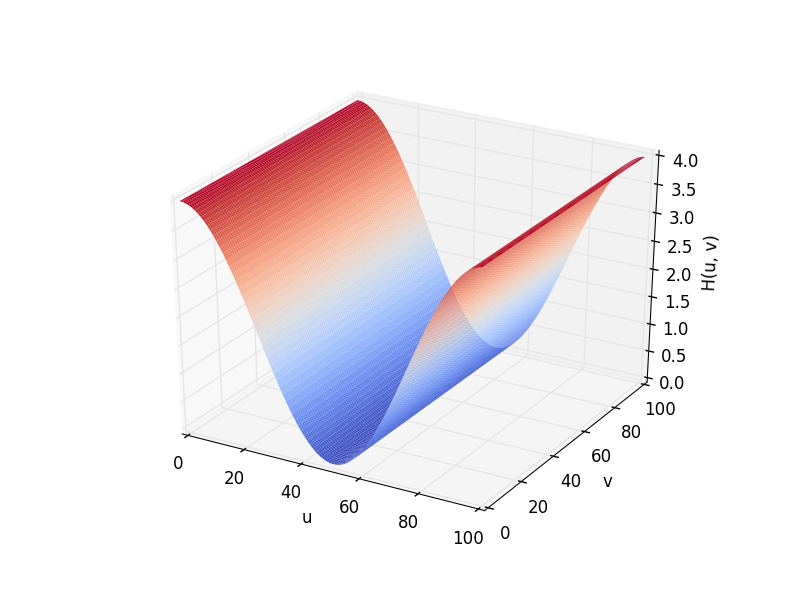
\includegraphics[width=420pt]{exercise-1-4.png}
	\caption{$H(u, v)$ where $M = N = 100$}
	\label{fig:Huv}
\end{figure}


% -------------------- Programming Tasks ------------------------
\section{Programming Tasks}
% -------------------- Fourier Transform ------------------------
\subsection{Fourier Transform}
% -------------------- Results ------------------------
\subsubsection{Results}
\begin{figure}[H]
	\centering
	% pt = px * 72 / DPI
	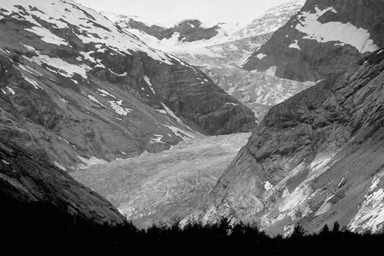
\includegraphics[width=288pt]{../img/02.png}
	\caption{The original image}
\end{figure}

\begin{figure}[H]
	\centering
	% pt = px * 72 / DPI
	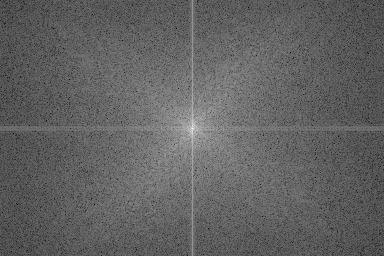
\includegraphics[width=288pt]{../result/dft-spectrum.png}
	\caption{The centered Fourier spectrum}
\end{figure}

\begin{figure}[H]
	\centering
	% pt = px * 72 / DPI
	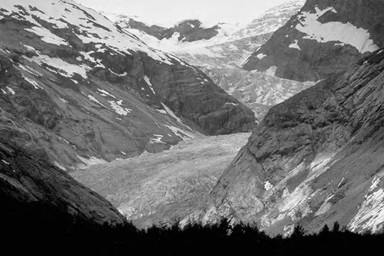
\includegraphics[width=288pt]{../result/dft-double.png}
	\caption{The real part of the IDFT of the DFT}
\end{figure}


% -------------------- Discussion ------------------------
\subsubsection{Discussion}

\indent Since the data obtained from the original image is real, and

$$\mathfrak{F}^{-1}[\mathfrak{F}[f(x,y)]] \equiv f(x,y)$$

if we take the DFT of the original image, then apply IDFT, theoretically the real part of the result is the same as the original image. In practice, however, there might be some small errors caused by the limited presicion of floating numbers.

To accelerate the calculation, we can pre-compute the discrete fourier transform  matrix. Let $N$ be the size of the 1D vector $\mathbf{f}$ that will be transformed, the discrete fourier transform matrix is:

$$\mathbf{W}_{x,y} = e^{\frac{j2\pi xy}{N}}$$

Then the discrete fourier transform $\mathbf{F} = \mathbf{W} \mathbf{f}$, that is, the dot product of the transform matrix and the original vector. Using the separability of the fourier transform, for a $M \times N$ matrix $f$, its discrete fourier transform $\mathbf{F} = \mathbf{W_M} \mathbf{f} \mathbf{W_N}$, where $\mathbf{W_M}$ and $\mathbf{W_N}$ are discrete fourier transform matrices for vectors of size $M$ and $N$.

Similarly, the transform matrix for discrete inverse fourier transform is:

$$\mathbf{W^i}_{x,y} = e^{\frac{-j2\pi xy}{N}}$$

The 1D transform is $f = \frac{1}{N} \mathbf{W^i} \mathbf{F}$, the 2D transform is $f = \frac{1}{MN} \mathbf{W^i_M} \mathbf{F} \mathbf{W^i_N}$


% -------------------- Algorithm ------------------------
\subsubsection{Algorithm}

\begin{algorithm}[H]
\centering
\caption{Discrete Fourier Transform}
  \begin{algorithmic}[1]
    \Function{dft2d}{$input\_img$, flags}
      \State $M$ = number of rows in $input\_img$
      \State $N$ = number of columns in $input\_img$
      \If{flags = 1}
	      \State $\mathbf{W_M}$ = \Call{dftmtx}{$M$}
	      \State $\mathbf{W_N}$ = \Call{dftmtx}{$N$}
	      \State \Return $\mathbf{W_M} \mathbf{f} \mathbf{W_N}$
      \Else
	      \State $\mathbf{W^i_M}$ = \Call{idftmtx}{$M$}
	      \State $\mathbf{W^i_N}$ = \Call{idftmtx}{$N$}
	      \State \Return $\frac{1}{MN} \mathbf{W^i_M} \mathbf{f} \mathbf{^iW_N}$
      \EndIf
    \EndFunction
    \\
    \Function{dftmtx}{$N$}
      \State \Return Matrix $\mathbf{W}_{x,y} = e^{\frac{j2\pi xy}{N}}$
    \EndFunction
    \\
    \Function{idftmtx}{$N$}
      \State \Return Matrix $\mathbf{W_i}_{x,y} = e^{\frac{-j2\pi xy}{N}}$
    \EndFunction
  \end{algorithmic}
\end{algorithm}

% -------------------- Fast Fourier Transform ------------------------

\subsection{Fast Fourier Transform}

% -------------------- Results ------------------------
\subsubsection{Results}
\begin{figure}[H]
	\centering
	% pt = px * 72 / DPI
	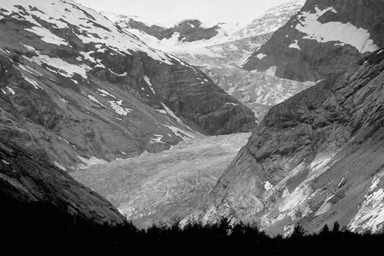
\includegraphics[width=288pt]{../img/02.png}
	\caption{The original image}
\end{figure}

\begin{figure}[H]
	\centering
	% pt = px * 72 / DPI
	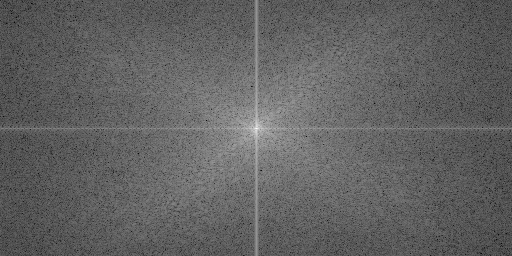
\includegraphics[width=384pt]{../result/fft-spectrum.png}
	\caption{The centered Fourier spectrum}
\end{figure}

\begin{figure}[H]
	\centering
	% pt = px * 72 / DPI
	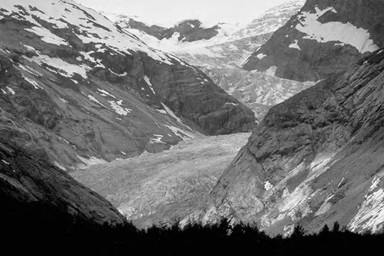
\includegraphics[width=288pt]{../result/fft-double.png}
	\caption{The real part of the IDFT of the DFT}
\end{figure}

% -------------------- Discussion ------------------------
\subsubsection{Discussion}

Here I use the Cooley–Tukey algorithm to compute the fast fourier transform, which requires the length of the input vector to be power of 2.

The recursive version is easy to implement, but it takes a bit too long. To accelerate it, we can rewrite it into a iterative version. Since in each step, the odd parts in subproblems are actually the latter half of all subproblems of the previous step, and the even parts the former half, we can concatenate all odd parts and all even parts, and use the symmetry of the twiddle factor to vectorize the butterfly operation.

In addition, when the length of the input is smaller than a cut-off value (on my computer, 16), then it could be faster to use the vectorized DFT implemented before. We can use it to optimize for our smaller subproblems.

Because of the seperability of DFT, The 2D FFT can be obtained by simply applying the 1D FFT over each row of the matrix, and then apply it over each column.

Since

$$MNf^*(x,y) = \sum_{u=0}^{M-1}\sum_{v=0}^{N-1} F^*(u, v) e^{-j2\pi (ux/M + vy/N)}$$

to implement the IFFT, we can compute the 2D forward FFT for the complex conjugate of the data, divide the result by $MN$, and then take the complex conjugate again.

% -------------------- Algorithm ------------------------
\subsubsection{Algorithm}

\begin{algorithm}[H]
\centering
\caption{2D Fast Fourier Transform}
  \begin{algorithmic}[1]
    \Function{fft2d}{$input\_img$, flags}
      \If{flags == 1}
         \State Apply \Call{fft}{} over each row of $input\_img$
         \State Apply \Call{fft}{} over each column of $input\_img$
         \State \Return The transformed matrix
      \Else
         \State $output\_img$ = the complex conjugate of $input\_img$
         \State $output\_img$ = \Call{fft2d}{$input\_img$, -1}
         \State \Return the complex conjugate of $output\_img$
      \EndIf
    \EndFunction
  \end{algorithmic}
\end{algorithm}

\begin{algorithm}[H]
\caption{1D Fast Fourier Transform(recursive)}
  \begin{algorithmic}[1]
    \Function{fft}{$x$}
      \If{The length of $x$ == 1}
         \Return $x$
      \Else
         \State $even$ = elements of $x$ with even indices
         \State $odd$ = elements of $x$ with even indices
         \State $even$ = \Call{fft}{$even$}
         \State $odd$ = \Call{fft}{$odd$}
         \State $coff$ = $\mathbf{W}_{x} = e^{\frac{j2\pi x}{N}}$
         \State $first$ = $even$ + $coff$ * $odd$
         \State $second$ = $even$ - $coff$ * $odd$
         \State \Return concatenation of $first$ and $second$
      \EndIf
    \EndFunction
  \end{algorithmic}
\end{algorithm}

\begin{algorithm}[H]
\caption{1D Fast Fourier Transform (iterative)}
  \begin{algorithmic}[1]
    \Function{fft}{$x$}
      \While{$x$ is not a $N \times 1$ vector}
         \State $m$ = number of rows in $x$
         \State $even$ = first half of columns of $x$
         \State $odd$ = second half of columns of $x$
         \State $coff$ = $\mathbf{W}_{x} = e^{\frac{j\pi x}{N}}$
         \Comment Because of the concatenation, $m = 2N$, cancels out $2$
         \State $twiddle$ = mutiply each column of $odd$ by $coff$
         \State $x =$ concatenation of $even + twiddle$ and $even -  twiddle$
      \EndWhile
      \State\Return $x$
    \EndFunction
  \end{algorithmic}
\end{algorithm}

% -------------------- Spatial Filtering ------------------------
\subsection{Filtering in the Frequency Domain}

% -------------------- Results ------------------------
\subsubsection{Results}

\begin{figure}[H]
	\centering
		\[ \begin{bmatrix}
			-1 & -1 & -1 \\
			-1 &  8 & -1 \\
			-1 & -1 & -1
		\end{bmatrix} \]
\caption{Laplacian filter}
\end{figure}

\begin{figure}[]
	\centering
	% pt = px * 72 / DPI
	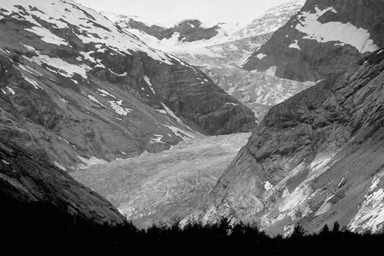
\includegraphics[width=288pt]{../img/02.png}
	\caption{The original image}
\end{figure}

\begin{figure}[]
	\centering
	% pt = px * 72 / DPI
	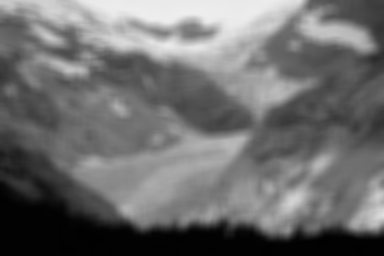
\includegraphics[width=288pt]{../result/average-11-11.png}
	\caption{Smoothed image with $11 \times 11$ averaging filter}
\end{figure}

\begin{figure}[]
	\centering
	% pt = px * 72 / DPI
	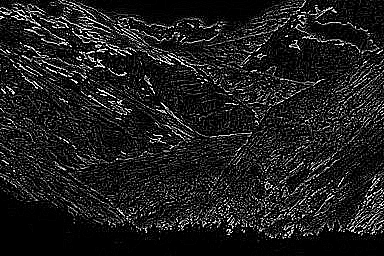
\includegraphics[width=288pt]{../result/laplacian.png}
	\caption{Image filtered with $3 \times 3$ Laplacian filter}
\end{figure}

\begin{description}
\item[Note] \hfill \\
To obtain a sharpened image with the result of a laplacian filter, we can combine the original image with the filtered result. Because the laplacian filter used here has a positive center, the sharpened image can be produced by:

$$g(x,y) = f(x, y) + laplacian(x, y)$$

where $g(x, y)$, $f(x, y)$, and $laplacian(x, y)$ are intensity values at the pixels of coordinate $(x, y)$ in the sharpened image, original image, and the laplacian filtered image, respectively.
\end{description}


% ---------------------- Discussion ---------------------------
\subsubsection{Discussion}
Since in the implementation, the array storing the input of the fourier transform doesn't support negative indices, the filter is actually translated by $(\frac{m}{2}, \frac{n}{2})$. Therefore the result needs to be cropped back after reversing this translation.

% ---------------------- Algorithm ---------------------------
\subsubsection{Algorithm}

\begin{description}
\item[Note] \hfill \\
I use the duplicate of borders to pad the input before filtering, and then crop out the result to avoid the inconsistency around the borders.
\end{description}

\begin{algorithm}[]
\centering
\caption{Filter}
  \begin{algorithmic}[1]
    \Function{filter2d\_freq}{$input\_img, filter$}
     \State $M, N$ = height and width of $input\_img$
     \State $m, n$ = height and width of $filter$
     \State $P, Q$ = the nearest larger power of 2 of $M + m - 1$ and $N + n - 1$
     \State $f_p$ = $input\_img$ padded to the upper left corner of a $P \times Q$ zero matrix
     \State $h_p$ = $filter$ padded to the upper left corner of a $P \times Q$ zero matrix
	 \State $F_{uv}$ = \Call{dft2d}{$f_p$, 1}
	 \State $H_{uv}$ = \Call{dft2d}{$h_p$, 1}
	 \State $G_{uv}$ = $F_{uv} H_{uv}$
     \State $result$ = The real part of \Call{dft2d}{$G_{uv}$, $-1$}
     \State \Return The image cropped from $result$, starting from $(\frac{m}{2}, \frac{n}{2})$
    \EndFunction
  \end{algorithmic}
\end{algorithm}

\bibliographystyle{acm}

\end{document}